% pandoc-xnos: cleveref fakery
\newcommand{\plusnamesingular}{}
\newcommand{\starnamesingular}{}
\newcommand{\xrefname}[1]{\protect\renewcommand{\plusnamesingular}{#1}}
\newcommand{\Xrefname}[1]{\protect\renewcommand{\starnamesingular}{#1}}
\providecommand{\cref}{\plusnamesingular~\ref}
\providecommand{\Cref}{\starnamesingular~\ref}
\providecommand{\crefformat}[2]{}
\providecommand{\Crefformat}[2]{}

% pandoc-xnos: cleveref formatting
\crefformat{figure}{fig.~#2#1#3}
\Crefformat{figure}{Figure~#2#1#3}

\hypertarget{introduction}{%
\section{Introduction}\label{introduction}}

Ecological networks are a useful way to think about ecological systems
in which species or organisms interact (Heleno et al. 2014; Poisot et
al. 2016c; Delmas et al. 2018), and recently there has been an explosion
of interest in their dynamics across large temporal scales (Tylianakis
\& Morris 2017; Baiser et al. 2019), and especially along environmental
gradients (Trøjelsgaard \& Olesen 2016; Pellissier et al. 2017). As
ecosystems and climates are changing rapidly, networks are at risk of
unravelling: for example by invasion of destabilizing exotic species
them (Strong \& Leroux 2014; Magrach et al. 2017), or by a ``rewiring''
of interactions among existing species (Guiden et al. 2019; Hui \&
Richardson 2019). Simulation studies suggest that knowing the shape of
the extant network is not sufficient (Thompson \& Gonzalez 2017), and
that it needs to be supplemented by additional data on the species in
the food web, climate, and climate projection.

This renewed interest in ecological networks has prompted several
methodological efforts. First, an expansion of the analytical tools to
study ecological networks and their variation in space (Poisot et al.
2012, 2015, 2017). Second, an improvement in large-scale
data-collection, through increased adoption of molecular biology tools
(Evans et al. 2016; Eitzinger et al. 2019) and crowd-sourcing of data
collection (Pocock et al. 2015; Bahlai \& Landis 2016; Roy et al. 2016).
Finally, a surge in the development of tools that allow us to
\emph{infer} species interactions (Morales-Castilla et al. 2015) based
on limited but complementary data on existing network properties (Stock
et al. 2017), species traits (Gravel et al. 2013; Desjardins-Proulx et
al. 2017; ~Brousseau et al. 2017; Bartomeus et al. 2016), and
environmental conditions (Gravel et al. 2018). These latter approaches
tend to perform well in data-poor environments (Beauchesne et al. 2016),
and can be combined through ensemble modeling or model averaging to
generate more robust predictions (Pomeranz et al. 2018). The task of
inferring interactions is particularly important because ecological
networks are difficult to adequately sample in nature (Banašek-Richter
et al. 2004; Gibson et al. 2011; Chacoff et al. 2012; Jordano 2016a).
The common goal to these efforts is to facilitate the prediction of
network structure, particularly over space {[}Poisot et al. (2016b);
Gravel et al. (2018); \textbf{MARINE FOODWEB}{]} and into the future
(Albouy et al. 2014), and to appraise the response of that structure to
possible environmental changes.

These disparate methodological efforts share another important trait:
their continued success depends on state-of-the art data management.
Novel quantitative tools demand a higher volume of network data; novel
collection techniques demand powerful data repositories; novel inference
tools demand easier integration between different types of data,
including but not limited to interactions, species traits, taxonomy,
occurrences, and local bioclimatic conditions. In short, advancing the
science of ecological networks requires us not only to increase the
volume of available data, but to pair these data with ecologically
relevant metadata. Such data should also be made available in a way that
facilitates programmatic interaction so that they can be used by
reproducible data analysis pipelines.

Poisot et al. (2016a) introduced \texttt{mangal.io} as a first step in
this direction. In the years since the tool was originally published, we
continued development of the data representation, amount and richness of
metadata, and digitized and standardized as much ecological data as we
could find. The second major release of this database contains over 1300
networks, 120000 interactions across close to 7000 taxa, and represents
what is to our best knowledge the most complete collection of species
interactions available. We seek to assess the fitness for purpose of
ecological networks at the global scale to support synthesis research.
Based on temporal and spatial biases in the description of some types of
interactions, we conclude that while there is an increasing amount of
available data, most of the planet's surface is poorly described. In
particular, Africa, South America, and most of Asia have very sparse
coverage. This suggests that the accuracy of synthesis efforts on the
worldwide structure or properties of ecological networks will have very
low predictive values within these areas, and reinforces the need to
digitize available information, but also prioritize sampling towards
these locations.

\textbf{Main question} Here we address the question of what we can and
cannot do with this large store of ecological network data.

\begin{itemize}
\tightlist
\item
  A major challenge to ecological synthesis is generalizing from samples
  to the behaviour of ecological systems
\item
  two obstacles to such generalizing in ecological systems: data
  coverage and data quality

  \begin{itemize}
  \tightlist
  \item
    data coverage: are data collected from every relevant system?
  \item
    data quality: are data fit-for-purpose? Two particular aspects of
    quality

    \begin{itemize}
    \tightlist
    \item
      taxonomic resolution
    \item
      sampling effort Synthesizing ecological data presents important
      challenges and also some exciting opportunities. Mangal is well
      suited to offer such opportunities in the study of ecological
      networks.
    \end{itemize}
  \end{itemize}
\end{itemize}

\hypertarget{global-trends-in-ecological-networks-description}{%
\section{Global trends in ecological networks
description}\label{global-trends-in-ecological-networks-description}}

\hypertarget{network-coverage-is-accelerating-but-spatially-biased}{%
\subsection{Network coverage is accelerating but spatially
biased}\label{network-coverage-is-accelerating-but-spatially-biased}}

\begin{figure}
\centering
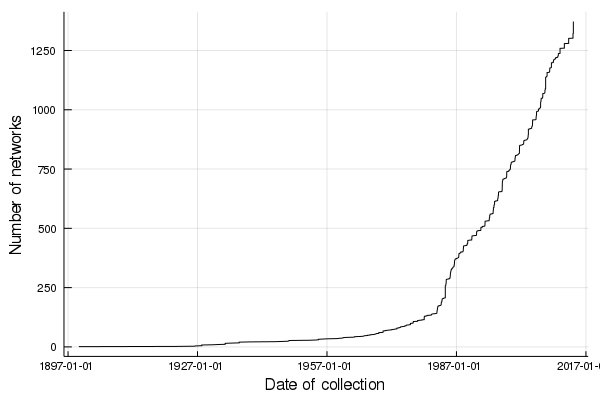
\includegraphics{figures/figure_01_a.png}
\caption{Cumulative number of ecological networks available in
\texttt{mangal.io} as a function of the date of collection. About 1000
unique networks have been collected between 1987 and 2017, a rate of
just over 30 networks a year. This temporal increase proceeds at
different rates for diferent types of networks; while the description of
food webs is more or less constant, the global acceleration in the
dataset is due to increased interest in host-parasite interactions
starting in the late 1970s, while mutualistic networks mostly started
being recorded in the early 2000s.\label{fig:temporal}}
\end{figure}

The earliest recorded ecological networks date back to the late
nineteenth century, with a strong increase in the rate of collection
around the 1980s (\xrefname{fig.}\cref{fig:temporal}). Although the
volume of available networks has increased over time, the sampling of
these networks in space has been uneven. In
\xrefname{fig.}\cref{fig:spatial}, we show that globally, network
collection is biased towards the Northern hemisphere, and than different
types of interactions have been sampled in different places. As such, it
is very difficult to find a spatial area of sufficiently large size in
which we have networks of predation, parasitism, and mutualism. The
inter-tropical zone is particularly data-poor, either because data
producers from the global South correctly perceive massive re-use of
their data by Western world scientists as a form of scientific
neo-colonialism (as advanced by Mauthner \& Parry 2013), thereby
providing a powerful incentive \emph{against} their publication, or
because ecological networks are subject to the same data deficit that is
affecting all fields on ecology in the tropics (Collen et al. 2008). As
Bruna (2010) identified almost ten years ago, improved data deposition
requires an infrastructure to ensure they can be repurposed for future
research, which we argue is provided by \texttt{mangal.io} for
ecological interactions.

\begin{figure}
\centering
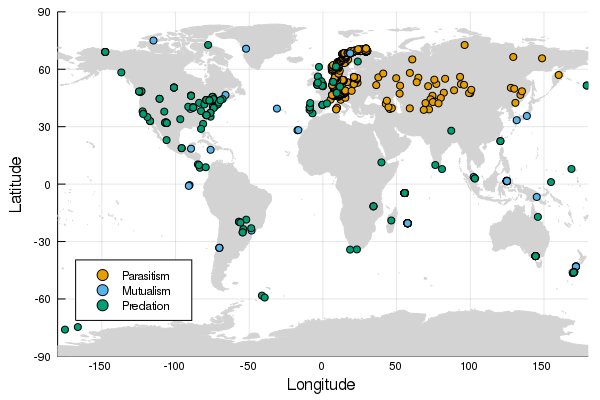
\includegraphics{figures/figure_01_c.png}
\caption{Each point on the map corresponds to a network with parasitic,
mutualistic, and predatory interactions. It is noteworty that the
spatial coverage of these types of interactions is uneven; the Americas
have almost no parasitic network, for example. Some places have barely
been studied at all, including Africa and Eastern Asia. This
concentration of networks around rich countries speaks to an inadequate
coverage of the diversity of landscapes on Earth.\label{fig:spatial}}
\end{figure}

\hypertarget{different-interaction-types-have-been-studied-in-different-biomes}{%
\subsection{Different interaction types have been studied in different
biomes}\label{different-interaction-types-have-been-studied-in-different-biomes}}

Whittaker (1962) suggested that natural communities can be partitioned
across biomes, largely defined as a function of their relative
precipitation and temperature. For all networks for which the latitude
and longitude was known, we extracted the value temperature (BioClim1,
yearly average) and precipitation (BioClim12, total annual) from the
WorldClim 2 data (Fick \& Hijmans 2017). Using these we can plot every
network on the map of biomes drawn by Whittaker (1962) (note that
because the frontiers between biomes are not based on any empirical or
systematic process, they have been omitted from this analysis). In
\xrefname{fig.}\cref{fig:biomes}, we show that even though networks
capture the overall diversity of precipitation and temperature, types of
networks have been studied in sub-spaces only. Specifically, parasitism
networks have been studied in colder and drier climates; mutualism
networks in wetter climates; predation networks display less of a bias.

\begin{figure}
\centering
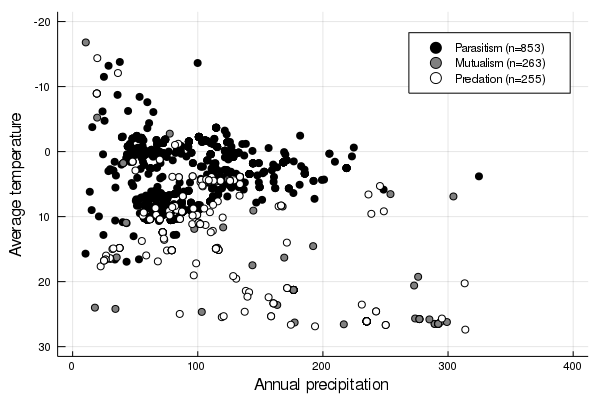
\includegraphics{figures/figure_02.png}
\caption{List of networks across in the space of biomes as originally
presented by Whittaker (1962). Predation networks, \emph{i.e.} food
webs, seem to have the most global coverage; parasitism networks are
restricted to low temperature and low precipitation biomes, congruent
with the majority of them being in Western Europe.\label{fig:biomes}}
\end{figure}

Scaling up this analysis to the 19 BioClim variables in Fick \& Hijmans
(2017), we extracted the position of every network in the bioclimatic
space, conducted a principal component analysis on the scaled
bioclimatic variables, and measured their distance to the centre of this
space (\(\mathbf{0}\)). This is a measurement of the ``rarity'' of the
bioclimatic conditions in which any networks were sampled, with larger
values indicating more unique combinations (the distance was ranged to
\(]0;1]\) for the sake of interpretation). As shown in
\xrefname{fig.}\cref{fig:ecc}, mutualistic interactions tend to have
values that are higher than both parasitism and predation, suggesting
that they have been sampled in more unique environments.

\begin{figure}
\centering
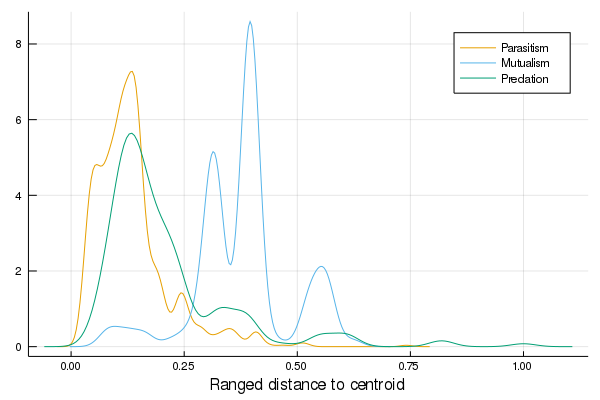
\includegraphics{figures/figure_05_b.png}
\caption{tk\label{fig:ecc}}
\end{figure}

\hypertarget{some-locations-on-earth-have-no-climate-analogue}{%
\subsection{Some locations on Earth have no climate
analogue}\label{some-locations-on-earth-have-no-climate-analogue}}

Climate analogue

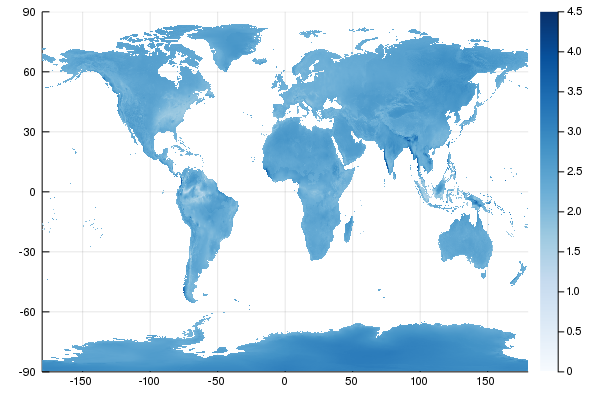
\includegraphics{figures/envirodistance_mutualism.png}
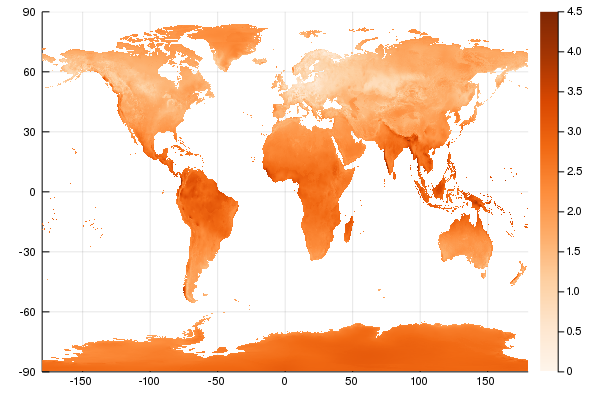
\includegraphics{figures/envirodistance_parasitism.png}
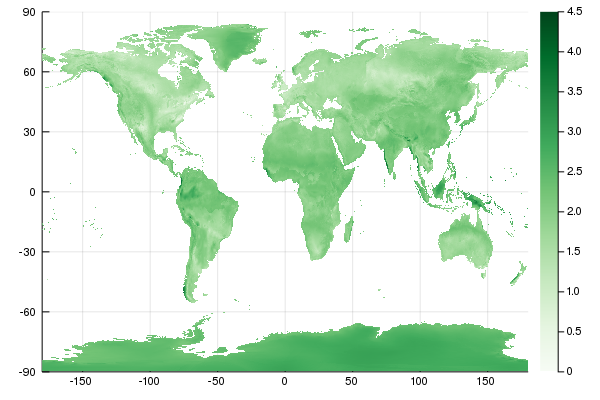
\includegraphics{figures/envirodistance_predation.png}

\hypertarget{conclusions}{%
\section{Conclusions}\label{conclusions}}

\hypertarget{data-quality-sampling-effort-and-taxonomy}{%
\subsection{Data quality: sampling effort and
taxonomy}\label{data-quality-sampling-effort-and-taxonomy}}

Jordano (2016b) -- importance of taxonomic resolution

Sampling effort and taxonomic detail are two very challenging but
important part of any ecological dataset. The datasets in Mangal
represent some of the most detailed studies of ecological networks
available. * measures of network structure may be particularly sensitive
to the amount of sampling effort * repeat sampling may be necessary to
capture a ``saturation'' of interactions. * we present some
visualization of the sampling coverage of Mangal {[}tk{]} * High
taxonomic resolution is difficult to achieve in ecology, especially
depending on the sampling method used (e.g.~gut contents vs
observations). We present a breakdown of the taxonomic resolution of
Mangal. * Ecological networks occur in various kinds, but they are not
all equally well sampled. We present a breakdown of the number of
parasitic, mutualistic and predator-prey networks sampled in Mangal

\hypertarget{can-we-predict-the-future-of-ecological-networks-under-climate-change}{%
\subsection{Can we predict the future of ecological networks under
climate
change?}\label{can-we-predict-the-future-of-ecological-networks-under-climate-change}}

Perhaps unsurprisingly, most of our knowledge on ecological networks is
derived from data that were collected after the 1990s
(\xrefname{fig.}\cref{fig:temporal}). This means that we have worryingly
little information on ecological networks before the acceleration of the
climate crisis, and therefore lack a robust baseline. Dalsgaard et al.
(2013) provide strong evidence that the extant shape of ecological
networks emerged in part in response to historical trends in climate
change. The lack of reference data before the acceleration of the
effects of climate change is of particular concern, as we may be
deriving intuitions on ecological network structure and assembly rules
from networks that are in the midst of important ecological
disturbances. Although there is some research on the response of
co-occurrence and indirect interactions to climate change (Araújo et al.
2011; Losapio \& Schöb 2017), these are a far cry from actual direct
interactions; similarly, the data on ``paleo-foodwebs'', \emph{i.e.}
from deep evolutionary time (Nenzén et al. 2014; Yeakel et al. 2014;
Muscente et al. 2018) represent the effect of more progressive change,
and may not adequately inform us about the future of ecological networks
under severe climate change. However, though we lack baselines against
which to measure the present, as a community we are in a position to
provide one for the future. Climate change will continue to have
important impacts on species distributions and interactions for at least
the next century {[}tk{]}. The Mangal database provides a structure to
organize and share network data, creating a baseline for future attempts
to monitor and adapt to biodiversity change.

Possibly more concerning is the fact that the spatial distribution of
sampled networks shows a clear bias towards the Western world,
specifically Western Europe and the Atlantic coasts of the USA and
Canada (\xrefname{fig.}\cref{fig:spatial}). This problem can be somewhat
circumvented by working on networks sampled in places that are close
analogues of those without direct information (almost all of Africa,
most of South America, a large part of Asia). However, ({\textbf{???}})
suggests that this approach will rapidly be limited: the diversity of
bioclimatic combinations on Earth leaves us with some areas lacking
suitable analogues. These regions are expected to bear the worst of the
socio-economical (\emph{e.g.} Indonesia) or ecological (\emph{e.g.}
polar regions) consequences of climate change {[}tk{]}. All things
considered, our current knowledge about the structure of ecological
networks at the global scale leaves us under-prepared to predict their
response to a warming world.

\hypertarget{what-purpose-are-global-ecological-network-data-fit-for}{%
\subsection{What purpose are global ecological network data fit
for?}\label{what-purpose-are-global-ecological-network-data-fit-for}}

This begs the question of \emph{what} can be achieved with our current
knowledge of ecological networks. \textbf{TK}

\hypertarget{active-development-and-data-contribution}{%
\subsection{Active development and data
contribution}\label{active-development-and-data-contribution}}

This is an open-source project: all data and all code supporting this
are available on the Mangal project GitHub organization. Our hope is
that the success of this project will encourage similar efforts within
other parts of the ecological community. In addition, we hope that this
project will encourage the recognition of the contribution that software
creators make to ecological research.

\hypertarget{references}{%
\section*{References}\label{references}}
\addcontentsline{toc}{section}{References}

\hypertarget{refs}{}
\leavevmode\hypertarget{ref-AlboVele14}{}%
\textbf{Albouy et al.} (2014). From projected species distribution to
food-web structure under climate change. \emph{Global Change Biology.}
20:730--41.

\leavevmode\hypertarget{ref-ArauRoze11}{}%
\textbf{Araújo et al.} (2011). Using species co-occurrence networks to
assess the impacts of climate change. \emph{Ecography.} 34:897--908.

\leavevmode\hypertarget{ref-BahlLand16}{}%
\textbf{Bahlai \& Landis}. (2016). Predicting plant attractiveness to
pollinators with passive crowdsourcing. \emph{Royal Society Open
Science.} 3:150677.

\leavevmode\hypertarget{ref-BaisGrav19}{}%
\textbf{Baiser et al.} (2019). Ecogeographical rules and the
macroecology of food webs. \emph{Global Ecology and Biogeography.} 0.

\leavevmode\hypertarget{ref-BanaCatt04}{}%
\textbf{Banašek-Richter et al.} (2004). Sampling effects and the
robustness of quantitative and qualitative food-web descriptors. \emph{J
Theor Biol.} 226:23--32.

\leavevmode\hypertarget{ref-BartGrav16}{}%
\textbf{Bartomeus et al.} (2016). A common framework for identifying
linkage rules across different types of interactions. \emph{Funct Ecol.}
30:1894--903.

\leavevmode\hypertarget{ref-BeauDesj16}{}%
\textbf{Beauchesne et al.} (2016). Thinking Outside the Box--predicting
Biotic Interactions in Data-poor Environments. \emph{Vie et milieu-life
and enVironment.} 66:333--42.

\leavevmode\hypertarget{ref-BrouGrav17}{}%
\textbf{Brousseau et al.} (2017). Trait-matching and phylogeny as
predictors of predator-prey interactions involving ground beetles.
\emph{Functional Ecology.}

\leavevmode\hypertarget{ref-Brun10}{}%
\textbf{Bruna}. (2010). Scientific Journals can Advance Tropical Biology
and Conservation by Requiring Data Archiving. \emph{Biotropica.}
42:399--401.

\leavevmode\hypertarget{ref-ChacVazq12}{}%
\textbf{Chacoff et al.} (2012). Evaluating sampling completeness in a
desert plant-pollinator network. \emph{J Anim Ecol.} 81:190--200.

\leavevmode\hypertarget{ref-CollRam08}{}%
\textbf{Collen et al.} (2008). The Tropical Biodiversity Data Gap:
Addressing Disparity in Global Monitoring. \emph{Tropical Conservation
Science.} 1:75--88.

\leavevmode\hypertarget{ref-DalsTroj13}{}%
\textbf{Dalsgaard et al.} (2013). Historical climate-change influences
modularity and nestedness of pollination networks. \emph{Ecography.}
36:1331--40.

\leavevmode\hypertarget{ref-DelmBess18}{}%
\textbf{Delmas et al.} (2018). Analysing ecological networks of species
interactions. \emph{Biological Reviews.}:112540.

\leavevmode\hypertarget{ref-DesjLaig17}{}%
\textbf{Desjardins-Proulx et al.} (2017). Ecological interactions and
the Netflix problem. \emph{PeerJ.} 5.

\leavevmode\hypertarget{ref-EitzAbre19}{}%
\textbf{Eitzinger et al.} (2019). Assessing changes in arthropod
predator--prey interactions through DNA-based gut content
analysis---variable environment, stable diet. \emph{Molecular Ecology.}
28:266--80.

\leavevmode\hypertarget{ref-EvanKits16}{}%
\textbf{Evans et al.} (2016). Merging DNA metabarcoding and ecological
network analysis to understand and build resilient terrestrial
ecosystems. \emph{Functional Ecology.}

\leavevmode\hypertarget{ref-FickHijm17}{}%
\textbf{Fick \& Hijmans}. (2017). WorldClim 2: new 1-km spatial
resolution climate surfaces for global land areas. \emph{Int J
Climatol.}:n/a--a.

\leavevmode\hypertarget{ref-GibsKnot11}{}%
\textbf{Gibson et al.} (2011). Sampling method influences the structure
of plant--pollinator networks. \emph{Oikos.} 120:822--31.

\leavevmode\hypertarget{ref-GravBais18}{}%
\textbf{Gravel et al.} (2018). Bringing Elton and Grinnell together: a
quantitative framework to represent the biogeography of ecological
interaction networks. \emph{Ecography.} 0.

\leavevmode\hypertarget{ref-GravPois13}{}%
\textbf{Gravel et al.} (2013). Inferring food web structure from
predator-prey body size relationships. Freckleton, ed. \emph{Methods in
Ecology and Evolution.} 4:1083--90.

\leavevmode\hypertarget{ref-GuidBart19}{}%
\textbf{Guiden et al.} (2019). Predator--Prey Interactions in the
Anthropocene: Reconciling Multiple Aspects of Novelty. \emph{Trends in
Ecology \& Evolution.} 0.

\leavevmode\hypertarget{ref-HeleGarc14}{}%
\textbf{Heleno et al.} (2014). Ecological networks: delving into the
architecture of biodiversity. \emph{Biol Lett.} 10.

\leavevmode\hypertarget{ref-HuiRich19}{}%
\textbf{Hui \& Richardson}. (2019). How to Invade an Ecological Network.
\emph{Trends in Ecology \& Evolution.} 34:121--31.

\leavevmode\hypertarget{ref-Jord16}{}%
\textbf{Jordano}. (2016a). Chasing Ecological Interactions. \emph{PLOS
Biol.} 14:e1002559.

\leavevmode\hypertarget{ref-Jord16a}{}%
\textbf{Jordano}. (2016b). Sampling networks of ecological interactions.
\emph{Functional Ecology.}

\leavevmode\hypertarget{ref-LosaScho17}{}%
\textbf{Losapio \& Schöb}. (2017). Resistance of plant--plant networks
to biodiversity loss and secondary extinctions following simulated
environmental changes. \emph{Functional Ecology.} 31:1145--52.

\leavevmode\hypertarget{ref-MagrHolz17}{}%
\textbf{Magrach et al.} (2017). Plant-pollinator networks in
semi-natural grasslands are resistant to the loss of pollinators during
blooming of mass-flowering crops. \emph{Ecography.}:n/a--a.

\leavevmode\hypertarget{ref-MautParr13}{}%
\textbf{Mauthner \& Parry}. (2013). Open Access Digital Data Sharing:
Principles, Policies and Practices. \emph{Social Epistemology.}
27:47--67.

\leavevmode\hypertarget{ref-MoraMati15}{}%
\textbf{Morales-Castilla et al.} (2015). Inferring biotic interactions
from proxies. \emph{Trends in Ecology \& Evolution.}

\leavevmode\hypertarget{ref-MuscPrab18}{}%
\textbf{Muscente et al.} (2018). Quantifying ecological impacts of mass
extinctions with network analysis of fossil communities.
\emph{PNAS.}:201719976.

\leavevmode\hypertarget{ref-NenzMont14}{}%
\textbf{Nenzén et al.} (2014). The Impact of 850,000 Years of Climate
Changes on the Structure and Dynamics of Mammal Food Webs. \emph{PLOS
ONE.} 9:e106651.

\leavevmode\hypertarget{ref-PellAlbo17}{}%
\textbf{Pellissier et al.} (2017). Comparing species interaction
networks along environmental gradients. \emph{Biol Rev Camb Philos Soc.}

\leavevmode\hypertarget{ref-PocoRoy15}{}%
\textbf{Pocock et al.} (2015). The Biological Records Centre: a pioneer
of citizen science. \emph{Biol J Linn Soc.} 115:475--93.

\leavevmode\hypertarget{ref-PoisBais16}{}%
\textbf{Poisot et al.} (2016a). mangal - making ecological network
analysis simple. \emph{Ecography.} 39:384--90.

\leavevmode\hypertarget{ref-PoisCana12}{}%
\textbf{Poisot et al.} (2012). The dissimilarity of species interaction
networks. \emph{Ecol Lett.} 15:1353--61.

\leavevmode\hypertarget{ref-PoisGrav16}{}%
\textbf{Poisot et al.} (2016b). Synthetic datasets and community tools
for the rapid testing of ecological hypotheses. \emph{Ecography.}
39:402--8.

\leavevmode\hypertarget{ref-PoisGuev17}{}%
\textbf{Poisot et al.} (2017). Hosts, parasites and their interactions
respond to different climatic variables. \emph{Global Ecol
Biogeogr.}:n/a--a.

\leavevmode\hypertarget{ref-PoisStou15}{}%
\textbf{Poisot et al.} (2015). Beyond species: why ecological
interaction networks vary through space and time. \emph{Oikos.}
124:243--51.

\leavevmode\hypertarget{ref-PoisStou16}{}%
\textbf{Poisot et al.} (2016c). Describe, understand and predict: why do
we need networks in ecology? \emph{Funct Ecol.} 30:1878--82.

\leavevmode\hypertarget{ref-PomeThom18}{}%
\textbf{Pomeranz et al.} (2018). Inferring predator-prey interactions in
food webs. \emph{Methods in Ecology and Evolution.} 0.

\leavevmode\hypertarget{ref-RoyBaxt16}{}%
\textbf{Roy et al.} (2016). Focal Plant Observations as a Standardised
Method for Pollinator Monitoring: Opportunities and Limitations for Mass
Participation Citizen Science. \emph{PLOS ONE.} 11:e0150794.

\leavevmode\hypertarget{ref-StocPois17}{}%
\textbf{Stock et al.} (2017). Linear filtering reveals false negatives
in species interaction data. \emph{Scientific Reports.} 7:45908.

\leavevmode\hypertarget{ref-StroLero14}{}%
\textbf{Strong \& Leroux}. (2014). Impact of Non-Native Terrestrial
Mammals on the Structure of the Terrestrial Mammal Food Web of
Newfoundland, Canada. \emph{PLOS ONE.} 9:e106264.

\leavevmode\hypertarget{ref-ThomGonz17}{}%
\textbf{Thompson \& Gonzalez}. (2017). Dispersal governs the
reorganization of ecological networks under environmental change.
\emph{Nature Ecology \& Evolution.} 1:0162.

\leavevmode\hypertarget{ref-TrojOles16}{}%
\textbf{Trøjelsgaard \& Olesen}. (2016). Ecological networks in motion:
micro- and macroscopic variability across scales. \emph{Funct Ecol.}
30:1926--35.

\leavevmode\hypertarget{ref-TyliMorr17}{}%
\textbf{Tylianakis \& Morris}. (2017). Ecological Networks Across
Environmental Gradients. \emph{Annual Review of Ecology, Evolution, and
Systematics.} 48:25--48.

\leavevmode\hypertarget{ref-Whit62}{}%
\textbf{Whittaker}. (1962). Classification of Natural Communities.
\emph{Botanical Review.} 28:1--239.

\leavevmode\hypertarget{ref-YeakPire14}{}%
\textbf{Yeakel et al.} (2014). Collapse of an ecological network in
Ancient Egypt. \emph{PNAS.} 111:14472--7. 
